\documentclass[12pt]{report}
\usepackage[utf8]{inputenc}
\usepackage[T2A]{fontenc}
\usepackage[russian]{babel}

\usepackage{amsmath,amsfonts,amssymb,amsthm,mathtools}
\DeclarePairedDelimiter\abs{\lvert}{\rvert}

\usepackage{pgfplots}
\usepackage{filecontents}
\usepackage{indentfirst}
\usepackage{eucal}
\usepackage{enumitem}
% Для \abs{}
\usepackage{commath}
\usepackage{float}
\frenchspacing

% Для нормальных переносов
\sloppy

\usetikzlibrary{datavisualization}
\usetikzlibrary{datavisualization.formats.functions}

\usepackage[left=2cm,right=2cm, top=2cm,bottom=2cm,bindingoffset=0cm]{geometry}
% Для измененных титулов глав:
\usepackage{titlesec, blindtext, color} % подключаем нужные пакеты
\definecolor{gray75}{gray}{0.75} % определяем цвет
\newcommand{\hsp}{\hspace{20pt}} % длина линии в 20pt
% titleformat определяет стиль
\titleformat{\chapter}[hang]{\Huge\bfseries}{\thechapter\hsp\textcolor{gray75}{|}\hsp}{0pt}{\Huge\bfseries}

% plot
\usepackage{xcolor}
\usepackage{stmaryrd}
\usepackage{wasysym}
\usetikzlibrary{datavisualization}
\usetikzlibrary{datavisualization.formats.functions}

% листинги
\usepackage{listings}
\usepackage{graphicx}
\usepackage{caption}
\usepackage{textcomp}
\lstset{
    language = Python,
    basicstyle=\small\sffamily,
    numbers=left,
    numberstyle=\tiny,
    stepnumber=1,
    numbersep=5pt,
    showspaces=false,
    showstringspaces=false,
    showtabs=false,
    frame=single,
    tabsize=2,
    captionpos=t,
    breaklines=true,
    breakatwhitespace=false,
    escapeinside={\#*}{*)}
}
\captionsetup[lstlisting]{justification=raggedright, singlelinecheck=off}

\begin{document}
%\def\chaptername{} % убирает "Глава"
    \include{title}
    \tableofcontents

    % Введение
    \newpage
    \chapter*{Введение}
    \addcontentsline{toc}{chapter}{Введение}

    Многопоточность — способность центрального процессора (CPU) или одного ядра
    в многоядерном процессоре одновременно выполнять несколько процессов или
    потоков, соответствующим образом поддерживаемых операционной системой.

    Этот подход отличается от многопроцессорности, так как многопоточность
    процессов и потоков совместно использует ресурсы одного или нескольких ядер:
    вычислительных блоков, кэш-памяти ЦПУ или буфера перевода с преобразованием (TLB).

    В тех случаях, когда многопроцессорные системы включают в себя несколько полных блоков обработки,
    многопоточность направлена на максимизацию использования ресурсов одного ядра,
    используя параллелизм на уровне потоков или на уровне инструкций.

    Поскольку эти два метода являются взаимодополняющими,
    их иногда объединяют в системах с несколькими многопоточными ЦП
    и в ЦП с несколькими многопоточными ядрами.

    Многопоточная парадигма стала более популярной с конца 1990-х годов,
    поскольку усилия по дальнейшему использованию параллелизма на уровне инструкций застопорились.

    Смысл многопоточности — квазимногозадачность на уровне одного исполняемого процесса.
    Значит, все потоки процесса помимо общего адресного пространства имеют и общие дескрипторы файлов.
    Выполняющийся процесс имеет как минимум один (главный) поток.

    Многопоточность (как доктрину программирования) не следует путать ни с многозадачностью,
    ни с многопроцессорностью, несмотря на то, что операционные системы,
    реализующие многозадачность, как правило, реализуют и многопоточность.

    Достоинства многопоточности:

    \begin{itemize}
        \item облегчение программы посредством использования общего адресного пространства;
        \item меньшие затраты на создание потока в сравнении с процессами;
        \item повышение производительности процесса за счёт распараллеливания процессорных вычислений;
        \item если поток часто теряет кэш, другие потоки могут продолжать
        использовать неиспользованные вычислительные ресурсы.
    \end{itemize}

    Недостатки многопоточности:

    \begin{itemize}
        \item несколько потоков могут вмешиваться друг в друга при совместном
        использовании аппаратных ресурсов \cite{Nemirovsky};
        \item с программной точки зрения аппаратная поддержка многопоточности
        более трудоемка для программного обеспечения \cite{Olukotun};
        \item проблема планирования потоков;
        \item специфика использования - вручную настроенные программы на ассемблере,
        использующие расширения MMX или AltiVec и выполняющие предварительные выборки данных,
        не страдают от потерь кэша или неиспользуемых вычислительных ресурсов.
        Таким образом, такие программы не выигрывают от аппаратной многопоточности
        и действительно могут иметь худшую производительность из-за конкуренции за общие ресурсы.
    \end{itemize}

    Однако несмотря на количество недостатков, перечисленных выше,
    многопоточная парадигма имеет большой потенциал на сегодняшний день,
    и при должном написании кода позволяет значительно ускорить однопоточные алгоритмы.

    \section*{Цель лабораторной работы}
    Целью данной лабораторной работы является изучение и реализация параллельных вычислений.

    \section*{Задачи лабораторной работы}
    В рамках выполнения работы необходимо решить следующие задачи:

    \begin{itemize}
        \item изучить понятие параллельных вычислений;
        \item реализовать последовательную и параллельную реализацию алгоритма нахождения определителя матрицы;
        \item сравнить временные характеристики реализованных алгоритмов экспериментально.
    \end{itemize}


    \chapter{Аналитическая часть}
    В данном разделе дано определение определителя матрицы и рассмотрены основные способы его нахождения.


    \section{Описание задачи}
    Определитель матрицы или просто определитель играет важную роль в решении систем линейных уравнений.
    Определитель матрицы $A$ обозначается как $\det{A}$, $\Delta{A}$, $\abs{A}$

    Сформулировать определение определителя матрицы можно на основе его свойств.
    Определителем вещественной матрицы называется функция $\det{}: \mathbb{R}^{n\times n} \rightarrow \mathbb{R}$,
    обладающая следующими свойствами:

    \begin{enumerate}
        \item $\det{(A)}$ - кососимметрическая функция строк (столбцов) матрицы $A$
        \item $\det{(A)}$ - полилинейная функция строк(столбцов) матрицы $A$
        \item $\det{(A)} = 1$, где $E$ - единичная $n \times n$-матрица
    \end{enumerate}


    \section{Нахождение определителя матрицы}
    Ниже описаны способы нахождения определителя матрицы размеров $1 \times 1$, $2 \times 2$, $3 \times 23$, $n \times 1n$.

    \subsection{Матрица $1 \times 1$}
    Для матрицы первого порядка значение детерминанта равно единственному элементу этой матрицы:

    \begin{equation}
        \label{eq:det_1x1}
        \Delta  = \abs{a_{11}} = a_{11}
    \end{equation}

    \subsection{Матрица $2 \times 2$}
    Для матрицы $2 \times 2$ определитель вычисляется следующим образом:

    \begin{equation}
        \label{eq:det_2x2}
        \Delta = \begin{vmatrix}
                     a & c \\
                     b & d
        \end{vmatrix} = ad - bc
    \end{equation}
    Абсолютное значение определителя $\abs{ad - bc}$ равно площади параллелограмма с вершинами
    $(0, 0), (a, b), (a + c, b + d), (c, d)$.

    \subsection{Матрица $3 \times 3$}
    Определитель матрицы $3 \times 3$ можно вычислить по формуле:
    \begin{multline}
        \label{eq:det_3x3}
        \Delta = \begin{vmatrix}
                     a_{11} & a_{12} & a_{13} \\
                     a_{21} & a_{22} & a_{23} \\
                     a_{31} & a_{32} & a_{33}
        \end{vmatrix} =
        a_{11} \cdot \begin{vmatrix}
                         a_{22} & a_{23} \\
                         a_{32} & a_{33}
        \end{vmatrix}
        -
        a_{12} \cdot \begin{vmatrix}
                         a_{21} & a_{23} \\
                         a_{31} & a_{33}
        \end{vmatrix}
        +
        a_{13} \cdot \begin{vmatrix}
                         a_{21} & a_{22} \\
                         a_{31} & a_{32}
        \end{vmatrix}
        = \\
        a_{11}a_{22}a_{33} - a_{11}a_{23}a_{32} - a_{12}a_{21}a_{33} +
        a_{12}a_{23}a_{31} + a_{13}a_{21}a_{32} - a_{13}a_{22}a_{31}
    \end{multline}

    Определитель матрицы, составленной из векторов $a, b, c$ представляет
    собой объём параллелепипеда, натянутого на вектора $a, b, c$.

    \subsection{Матрица $n \times n$}
    В общем случае, для матриц $n \times n$, где $n > 2$ определитель можно вычислить,
    применив следующую рекурсивную формулу:

    \begin{equation}
        \label{eq:det_nxn}
        \Delta =
        \sum\limits_{j = 1}^{n} (-1)^{1 + j} \cdot a_{1j} \cdot M_{j}^{-1}
        , \text{ где} M_{j}^{-1} - \text{дополнительный минор к элементу} a_{ij}
    \end{equation}

    В данной лабораторной работе стоит задача распараллеливания алгоритма нахождения определителя матрицы.
    Так как каждое слагаемое для вычисления итогового определителя
    вычисляется независимо от других и матрица не изменяется, для параллельного вычисления определителя
    было решено распределять задачу вычисления слагаемых между потоками.


    \section{Вывод}
    Обычный алгоритм нахождения определителя матрицы размера $n \times n$ независимо вычисляет слагаемые
    для нахождения итогового определителя, что дает возможность для реализации параллельного варианта алгоритма.
    \newpage


    \chapter{Конструкторская часть}
    Данный раздел содержит требования к разрабатываемому ПО,
    схемы алгоритмов, реализуемых в работе
    (Стандартный рекурсивный алгоритм нахождения определителя,
    алгоритм с использованием потоков и распределение слагаемых между потоками)
    и теоретический рассчет повышения эффективности исполнения алгоритма по времени.


    \section{Требования к программному обеспечению}
    Требования, выдвигаемые к разрабатываемому ПО:
    \begin{itemize}
        \item входные данные - размер матрицы (целое число), ее элементы (вещественные числа);
        \item выходные данные - определитель матрицы (вещественное число).
    \end{itemize}


    \section{Схемы алгоритмов}
    В данном пункте раздела представлены схемы реализуемых в работе алгоритмов.

    \subsection{Схема классического алгоритма}
    На рисунке~\ref{img:count_det} представлена схема рекурсивного алгоритма нахождения определителя.

    \begin{figure}[H]
        \centering
        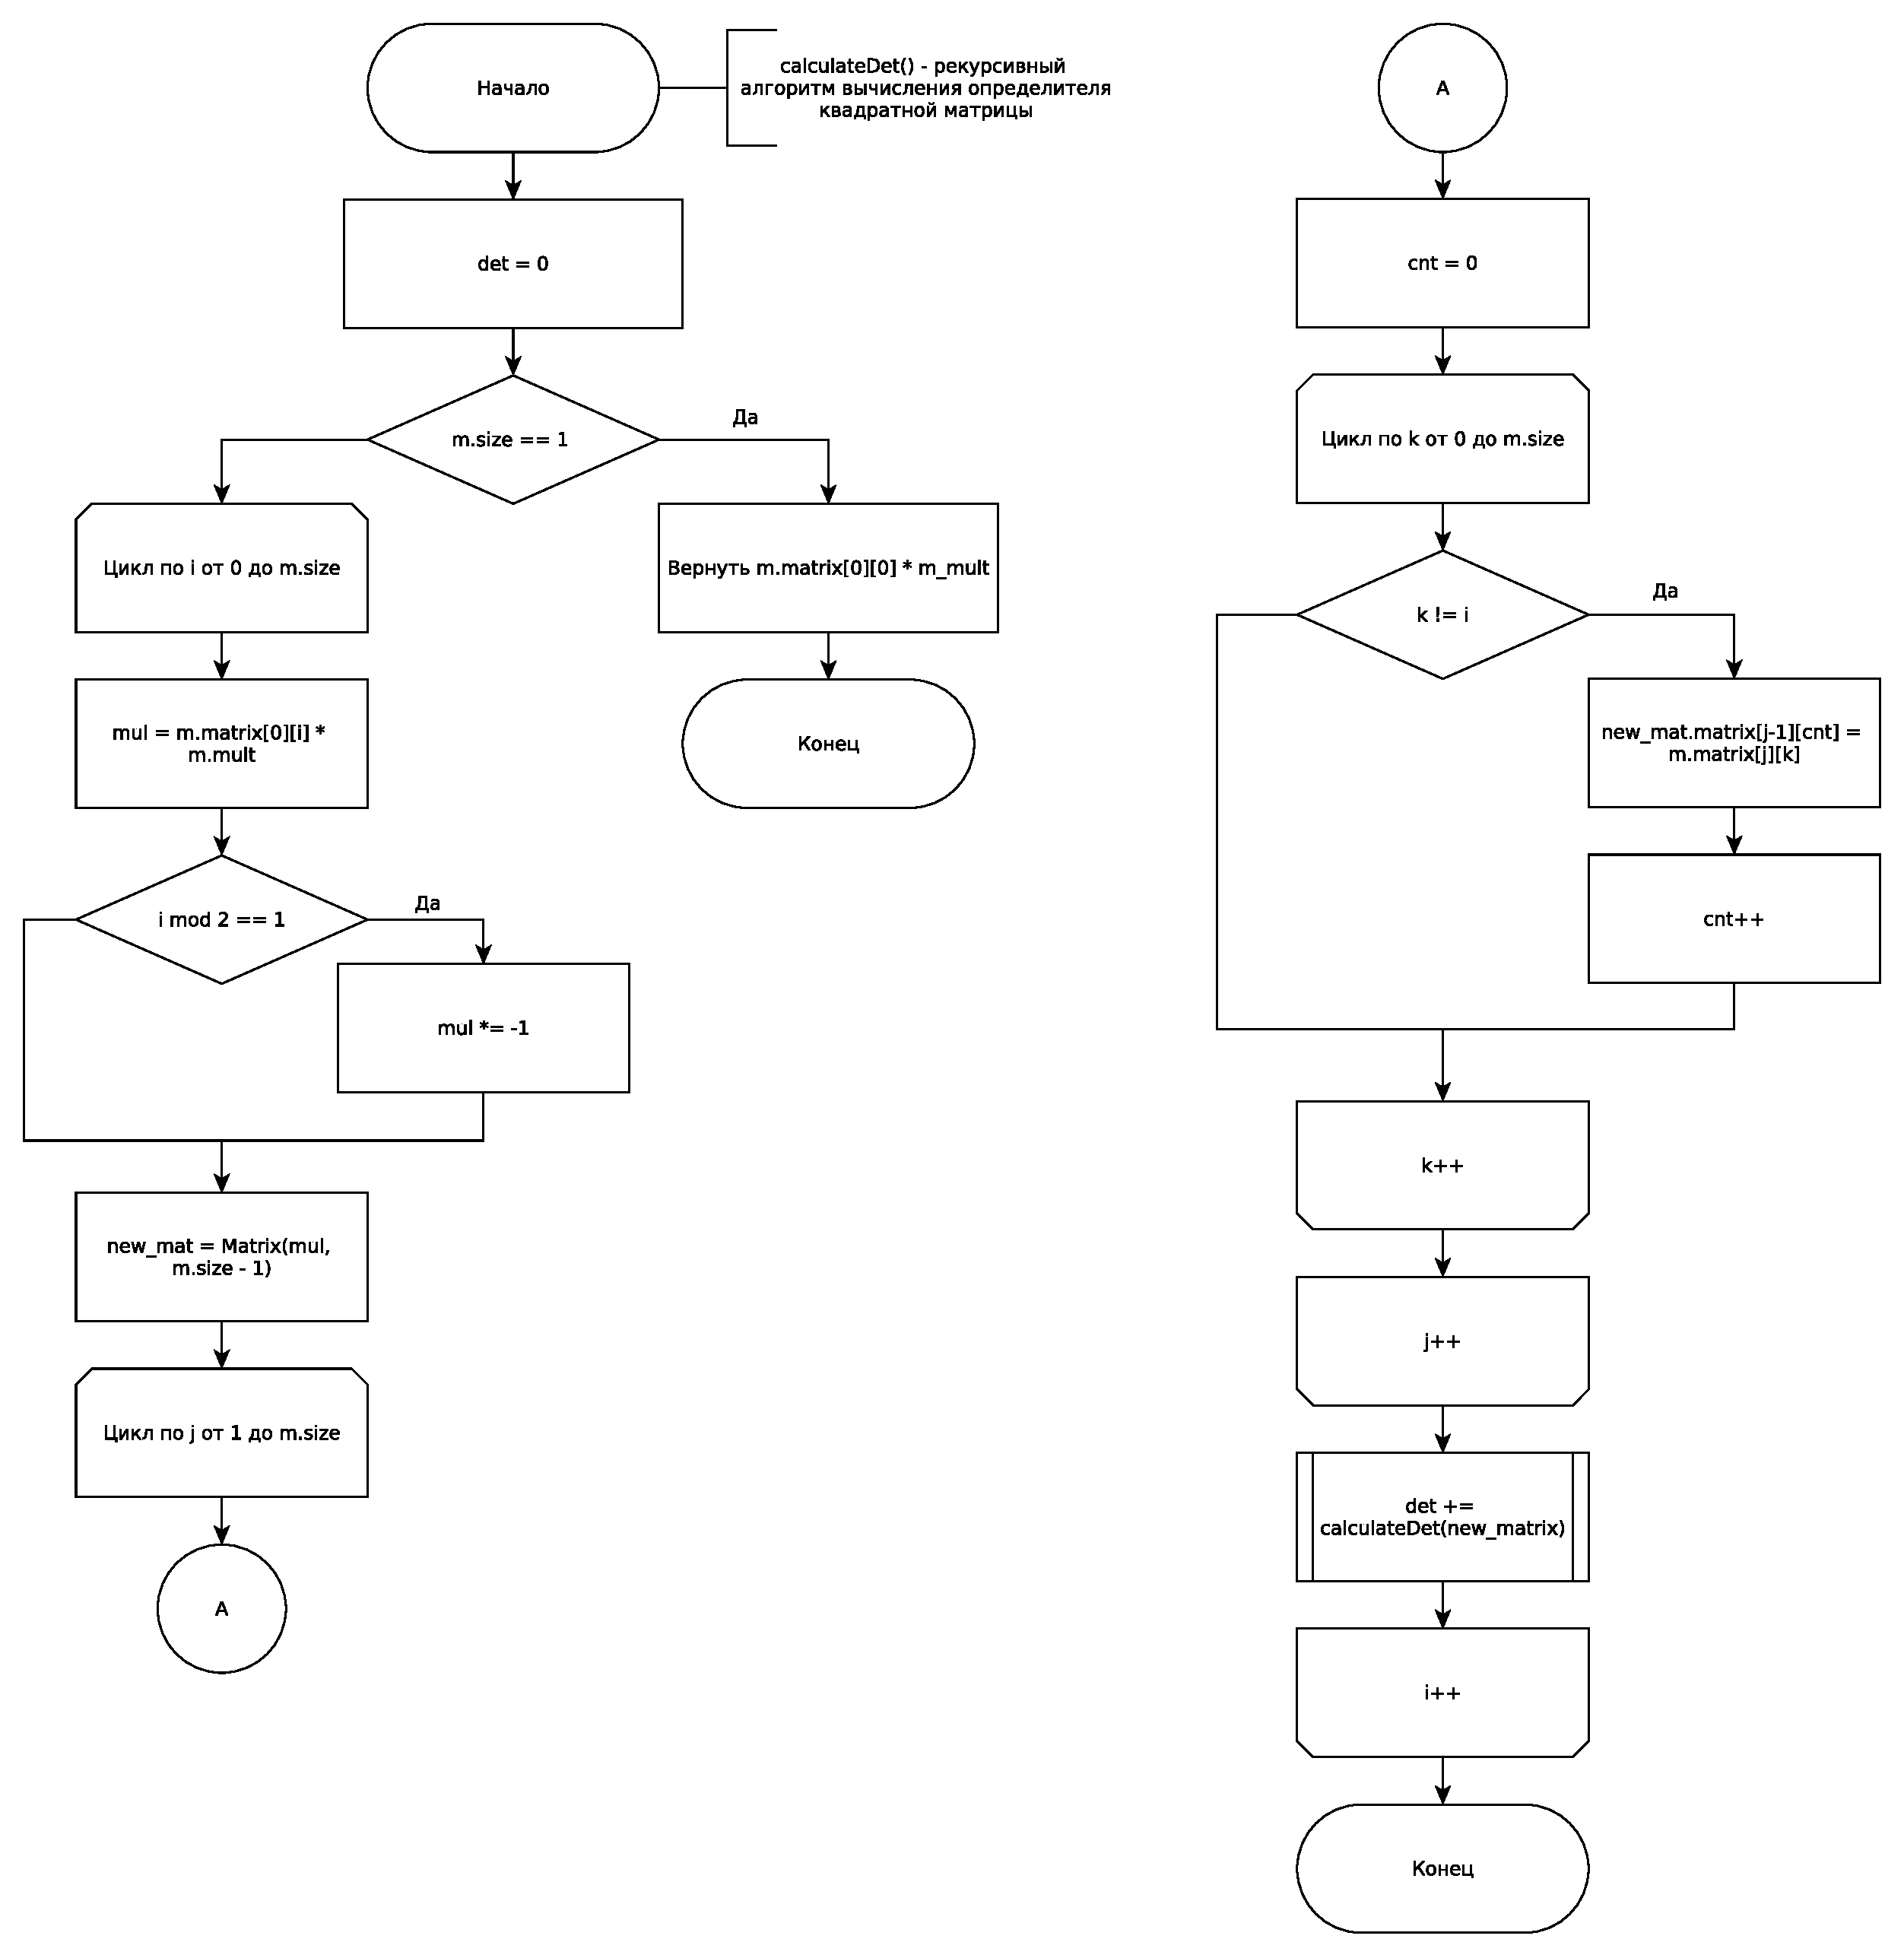
\includegraphics[width=1\linewidth]{img/count_det}
        \caption{
            Схема рекурсивного алгоритма нахождения определителя
        }
        \label{img:count_det}
    \end{figure}

    На рисунке~\ref{img:thread_schema} представлена схема алгоритма подсчета слагаемых итогового определителя матрицы
    при использовании потоков.

    \begin{figure}[H]
        \centering
        \includegraphics[width=0.85\linewidth]{img/thread_schema}
        \caption{
            Схема рекурсивного алгоритм нахождения определителя
        }
        \label{img:thread_schema}
    \end{figure}

    На рисунках~\ref{img:solver_1} -~\ref{img:solver_2} представлена схема алгоритма создания потоков,
    разделения задач между ними и нахождения итогового определителя матрицы.

    \begin{figure}[H]
        \centering
        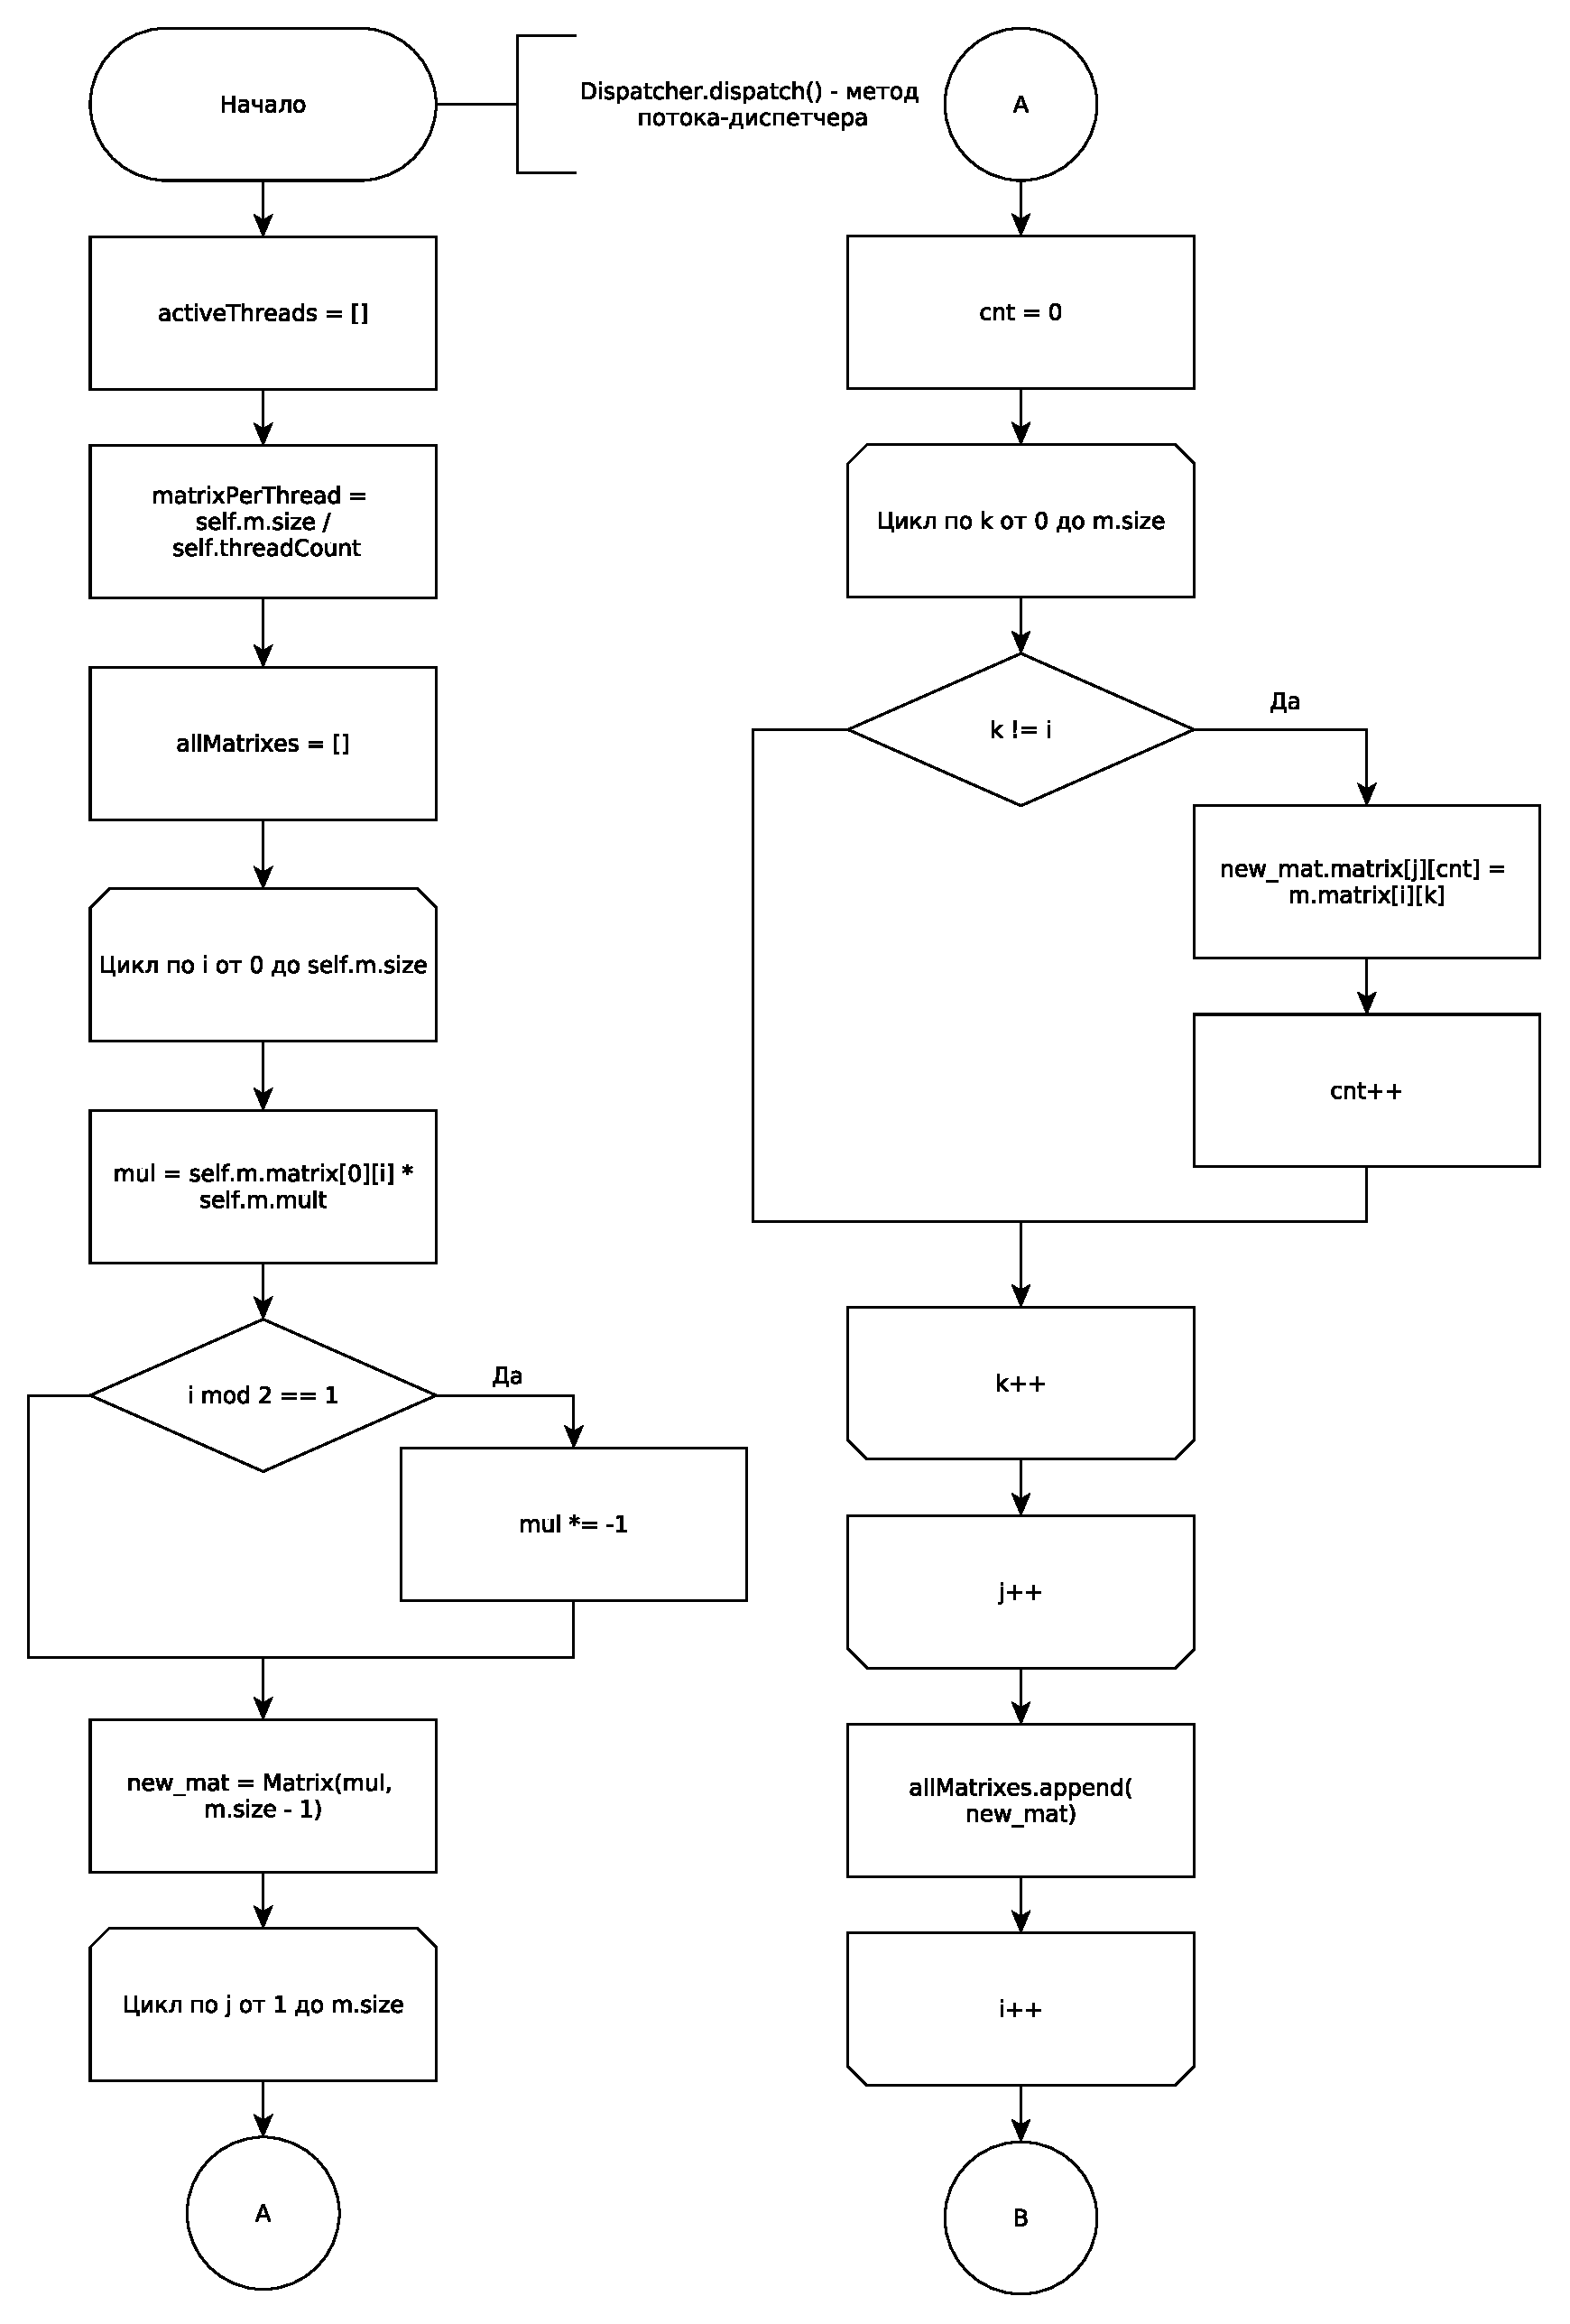
\includegraphics[width=0.85\linewidth]{img/solver_part_1}
        \caption{
            Схема рекурсивного алгоритм нахождения определителя
        }
        \label{img:solver_1}
    \end{figure}

    \begin{figure}[H]
        \centering
        \includegraphics[width=0.90\linewidth]{img/solver_part_2}
        \caption{
            Схема рекурсивного алгоритм нахождения определителя
        }
        \label{img:solver_2}
    \end{figure}

    \subsection{Теоретический рассчет эффективности по времени}

    При параллельном выполнении алгоритма изначальная матрица размером $n \times n$ делится на $n$ матриц
    со значением $mult = (-1)^{j + 1} \cdot a_{1j}$,
    где $j$ - номер элемента в первом ряду, для которого находится значение минора.
    Далее "подматрицы" равномерно распределяются между потоками для вычисления значения миноров.
    По мере работы потоки записывают результат в общий массив, и после окончания работы всех потоков
    определитель исходной матрицы считается как сумма элементов в общем массиве.

    При таком методе распараллеливания алгоритма для матрицы размером $n \times n$ эффективность
    алгоритма по времени исполнения должна повышаться примерно в $k$ раз, где $k$ - количество потоков,
    при $1 < k \leq n / 2$ или $k = n$.
    Однако при $ n / 2 < k < n$, время исполнения алгоритма не увеличится более чем в $n / 2$ раза,
    так как часть потоков будут искать два слагаемых итогового определителя, а часть - одно,
    в таком случае произойдет простой второй части потоков.


    \section{Вывод}
    В данном разделе на основе приведенных в аналитическом разделе теоретических данных
    были составлены схемы алгоритмов для реализации в технологической части.
    Были составлены схемы разделения вычисления определителя на потоки.
    Проведены теоретические расчеты эффективности параллельного алгоритма нахождения определителя.
    \newpage


    \chapter{Технологическая часть}
    Данный раздел содержит обоснование выбора языка и среды разработки, реализацию алгоритмов.


    \section{Средства реализации}
    Для реализации программы был выбран язык программирования Python~\cite{Python}.
    Такой выбор обусловлен следующими причинами:
    \begin{itemize}
        \item удобные средства для работы с потоками;
        \item обладает информативной документацией.
    \end{itemize}


    \section{Реализация алгоритмов}
    В листингах~\ref{code:normal} -~\ref{code:parallel} представлены
    реализации рассматриваемых алгоритмов.

    \begin{lstlisting}[caption=Рекурсивный алгоритм, label={code:normal}]
        def calculateSum(m: Matrix):
    s = 0
    if m.size == 2:
        return (m.matrix[0][0] * m.matrix[1][1] - m.matrix[0][1] * m.matrix[1][0]) * m.mult

    for i in range(m.size):
        mul = m.matrix[0][i] * m.mult
        if i % 2 == 1:
            mul *= -1

        size = m.size - 1
        matrix = []

        for j in range(1, m.size):
            matrix.append([])
            for k in range(m.size):
                if k != i:
                    matrix[-1].append(m.matrix[j][k])

        s += calculateSum(Matrix(size, mul, matrix))
    return s
    \end{lstlisting}

    \begin{lstlisting}[caption=Параллельный алгоритм с делением на потоки\, класс Solver и функция calculateSumThreading,
        label={code:parallel}]
        def calculateSumThreading(matrixes, returnList: list):
    t = time.time()
    s = 0

    for m in matrixes:
        if m.size == 2:
            returnList.append((m.matrix[0][0] * m.matrix[1][1] - m.matrix[0][1] * m.matrix[1][0]) * m.mult)
            continue

        for i in range(m.size):
            mul = m.matrix[0][i] * m.mult
            if i % 2 == 1:
                mul *= -1

            size = m.size - 1
            matrix = []

            for j in range(1, m.size):
                matrix.append([])
                for k in range(m.size):
                    if k != i:
                        matrix[-1].append(m.matrix[j][k])

            s += calculateSum(Matrix(size, mul, matrix))
            # allMatrixes.append(Matrix(size, mul, matrix))

    returnList.append(s)
    # print(f'process {getpid()}, time {time.time() - t}')

class Solver:
    def __init__(self, matrix: Matrix = None):
        self.m = matrix
        if self.m is None:
            self.m = Matrix(10).randomize()

        self.threadCount = 1
        self.threadManager = Manager()
        self.returnList = self.threadManager.list()


    def solve(self):
        activeThreads = []
        matrixPerThread = self.m.size / self.threadCount
        allMatrixes = []

        for i in range(self.m.size):
            mul = self.m.matrix[0][i] * self.m.mult
            if i % 2 == 1:
                mul *= -1

            size = self.m.size - 1
            matrix = []

            for j in range(1, self.m.size):
                matrix.append([])
                for k in range(self.m.size):
                    if k != i:
                        matrix[-1].append(self.m.matrix[j][k])

            allMatrixes.append(Matrix(size, mul, matrix))

        startMatrix = 0
        threadTasksCount = []

        for i in range(self.threadCount):
            endMatrix = round(matrixPerThread * (i+1))
            # if endMatrix == startMatrix: break
            if i == self.threadCount - 1:
                threadMatrixes = allMatrixes[startMatrix:]
            else:
                threadMatrixes = allMatrixes[startMatrix:endMatrix]
            startMatrix = endMatrix
            activeThreads.append(
                Process(target=calculateSumThreading, args=(threadMatrixes, self.returnList,)))
            threadTasksCount.append(len(threadMatrixes))

        for thread in activeThreads:
            thread.start()
        for thread in activeThreads:
            thread.join()
        self.returnList = self.threadManager.list()

        return sum(self.returnList)
    \end{lstlisting}


    \section{Тестирование}
    В таблице~\ref{tab:tests} представлены использованные для тестирования методом "черного ящика" данные,
    были рассмотрены все возможные тестовые случаи.
    Все тесты пройдены успешно.

    \begin{table}[H]
        \begin{center}
            \captionsetup{justification=raggedleft, singlelinecheck=false}
            \caption[]{\label{tab:tests} Проведенные тесты}

            \begin{tabular}{|c|c|}
                \hline
                \rule[-1ex]{0pt}{2.5ex} Матрица & Определитель \\
                \hline
                \rule[-1ex]{0pt}{2.5ex} $\begin{pmatrix}
                                             0 & 0 \\
                                             0 & 0
                \end{pmatrix}$ & 0
                \\
                \hline
                \rule[-1ex]{0pt}{2.5ex} $\begin{pmatrix}
                                             1 & 0 & 0 \\
                                             0 & 1 & 0 \\
                                             0 & 0 & 1
                \end{pmatrix}$ & 1
                \\
                \hline
                \rule[-1ex]{0pt}{2.5ex}    $\begin{pmatrix}
                                                1 & 2 & 3  \\
                                                4 & 5 & 6  \\
                                                7 & 8 & 12
                \end{pmatrix}$ & -9
                \\
                \hline
                \rule[-1ex]{0pt}{2.5ex} $\begin{pmatrix}
                                             1  & 2  & 3  & 4  \\
                                             5  & 6  & 7  & 8  \\
                                             9  & 10 & 11 & 12 \\
                                             13 & 14 & 15 & 16
                \end{pmatrix}$ & 0
                \\
                \hline
            \end{tabular}
        \end{center}
    \end{table}


    \section{Вывод}
    В данном разделе были реализованы и протестированы алгоритмы нахождения определителя матрицы:
    обычный и параллельный.
    \newpage


    \chapter{Экспериментальная часть}
    В данном разделе сравниваются реализованные алгоритмы, дается сравнительная оценка затрат по времени.


    \section{Пример работы программы}
    Пример работы программы представлен на рисунках~\ref{fig:work_1}-\ref{fig:work_2}.
    \captionsetup{singlelinecheck=true}
    \begin{figure}[H]
        \centering
        \includegraphics[width=0.7\linewidth]{img/example_1}
        \caption{Пользовательский ввод матрицы}
        \label{fig:work_1}
    \end{figure}

    \begin{figure}[H]
        \centering
        \includegraphics[width=0.7\linewidth]{img/example_2}
        \caption{Автоматическая генерация матрицы заданного размера}
        \label{fig:work_2}
    \end{figure}


    \section{Технические характеристики}
    Технические характеристики устройства, на котором выполнялось тестирование:
    \begin{itemize}
        \item операционная система --- Windows~\cite{windows} 10 64-bit;
        \item оперативная память --- 16 Гб;
        \item процессор --- Intel(R) Core(TM) i5-7600 CPU @ 3.50GHz~\cite{i5}.
    \end{itemize}


    \section{Время выполнения алгоритмов}

    Время выполнения алгоритмов замерялось на автоматически генерируемых
    квадратных матрицах необходимого размера с использованием функции getrusage библиотеки resources.

    \begin{table}[h]
        \begin{center}
            \captionsetup{justification=raggedleft, singlelinecheck=false}
            \caption{\label{time} Время нахождения определителя матрицы при
            использовании разного количества потоков в микросекундах}
            \begin{tabular}{|c c c c c c c|}
                \hline
                Размерность & 1 п. & 2 п. & 4 п. & 8 п. & 16 п. & 32 п.
                \\
                \hline
                4 & 10  & 14  & 17  & 23  & 38  & 67  \\
                \hline
                5 & 10  & 14  & 17  & 23  & 38  & 68  \\
                \hline
                6 & 12  & 15  & 17  & 24  & 39  & 68  \\
                \hline
                7 & 22  & 19  & 21  & 25  & 40  & 72  \\
                \hline
                8 & 75  & 47  & 37  & 42  & 57  & 82  \\
                \hline
                9 & 529 & 306 & 304 & 164 & 155 & 182 \\
                \hline
            \end{tabular}
        \end{center}
    \end{table}

    На рисунке~\ref{img:graph} графически изображена зависимость
    времени работы алгоритма от размерности матрицы и количества потоков.

    \begin{figure}[H]
        \centering
        \includegraphics[width=0.8\linewidth]{img/graph}
        \caption{
            Зависимость времени работы алгоритма от размерности матрицы и количества потоков
        }
        \label{img:graph}
    \end{figure}

    Поскольку процессор на устройстве содержит 4 физических и логических ядра,
    эффективность алгоритма улучшается только при создании 4 и менее потоков.
    Как видно по графику~\ref{img:graph}, с 2 потоками алгоритм выполнялся практически
    в 2 раза быстрее, чем с 1 потоком.
    Аналогичная ситуация наблюдается при сравнении 4 и 2 потоков.


    \section{Вывод}
    В данном разделе были проведены измерения времени, требуемого на исполнение алгоритма.
    По результатам измерений видно, что с увеличением количества потоков скорость выполнения
    алгоритма увеличивается.
    Однако как только количество потоков становится равно количеству логических ядер процессора,
    временные затраты на выполнение алгоритма увеличиваются из-за времени, затрачиваемого на
    создание новых потоков.


    \newpage

    \addcontentsline{toc}{chapter}{Заключение}
    \chapter*{Заключение}
    В процессе выполнения лабораторной работы были изучены и реализованы последовательный и
    параллельный рекурсивные алгоритмы нахождения определителя матрицы.

    Было экспериментально вычислено реальное время выполнения выше обозначенных алгоритмов.
    В результате было выявлено, что распараллеливание алгоритма нахождения определителя
    матрицы позволяет увеличить скорость его выполнения при использовании количества потоков
    меньшего или равного количеству логических ядер процессора.


    \newpage
    \addcontentsline{toc}{chapter}{Литература}

    \bibliographystyle{utf8gost705u}  % стилевой файл для оформления по ГОСТу
    \bibliography{report_4}          % имя библиографической базы (bib-файла)

\end{document}